\chapter{Implementation}
\label{ch:implementation}

\section{HDL structure}
Implementation starts from the block diagram described in Chapter \ref{ch:design}, moving from that to laying out the HDL skeleton within Scala. Both Chisel bundles (collections of inputs and outputs used to define interfaces) and Chisel modules are Scala classes, so the layout of the code follows a standard Java/Scala package layout \cite{scala_style}. The top-level package is \txt{dev.joeyh.pio} (the author's domain is \txt{joeyh.dev}), containing the top-level \txt{PIO} module class, and the following sub-packages and files

\begin{itemize}
    \item \txt{execution} - The execution unit and sub-components
          \begin{itemize}
              \item \txt{ExecUnit} - The top-level execution unit
              \item \txt{Decode} - Instruction decoder
              \item \txt{ProgramCounter} - PC register
              \item \txt{Branch} - JUMP execution unit
              \item \txt{Move} - MOV/SET execution unit
              \item \txt{Wait} - WAIT execution unit
          \end{itemize}
    \item \txt{fifo} - FIFOs and reusable interface definitions
          \begin{itemize}
              \item \txt{Fifo} - The FIFO module and sub-components, used for both RX and TX FIFOs
              \item \txt{ProducerIO} - Bundle definition for FIFO producer
              \item \txt{ConsumerIO} - Bundle definition for FIFO consumer
          \end{itemize}
    \item \txt{shiftreg} - Shift registers
          \begin{itemize}
              \item \txt{ISR} - Input shift register
              \item \txt{OSR} - Output shift register
              \item \txt{ShiftRegIO} - Common shift register interface definitions
          \end{itemize}
    \item \txt{memory} - Shift registers
          \begin{itemize}
              \item \txt{CSR} - Control and status register file
              \item \txt{InstructionMem} - 32x16bit Instruction memory
              \item \txt{ScratchReg} - 32-bit scratch register
          \end{itemize}
    \item \txt{util} - Miscellaneous reusable components and utilities
          \begin{itemize}
              \item \txt{Random} - functions for generating random Chisel \txt{UInt}s, used for testing
              \item \txt{ReadWrite} - reusable read and write port interface definitions
          \end{itemize}
\end{itemize}

Some files contain one (or more) Chisel modules, while others contain bundle definitions that are designed to be reused accross multiple modules. Bundles as types is a great feature of Chisel, as it allows to abstract over them using the connection operators. The module hierarchy of the overall design from this is fairly flat, shown in Figure \ref{fig:hdl_hierarchy}.

\begin{figure}[H]
    \centering
    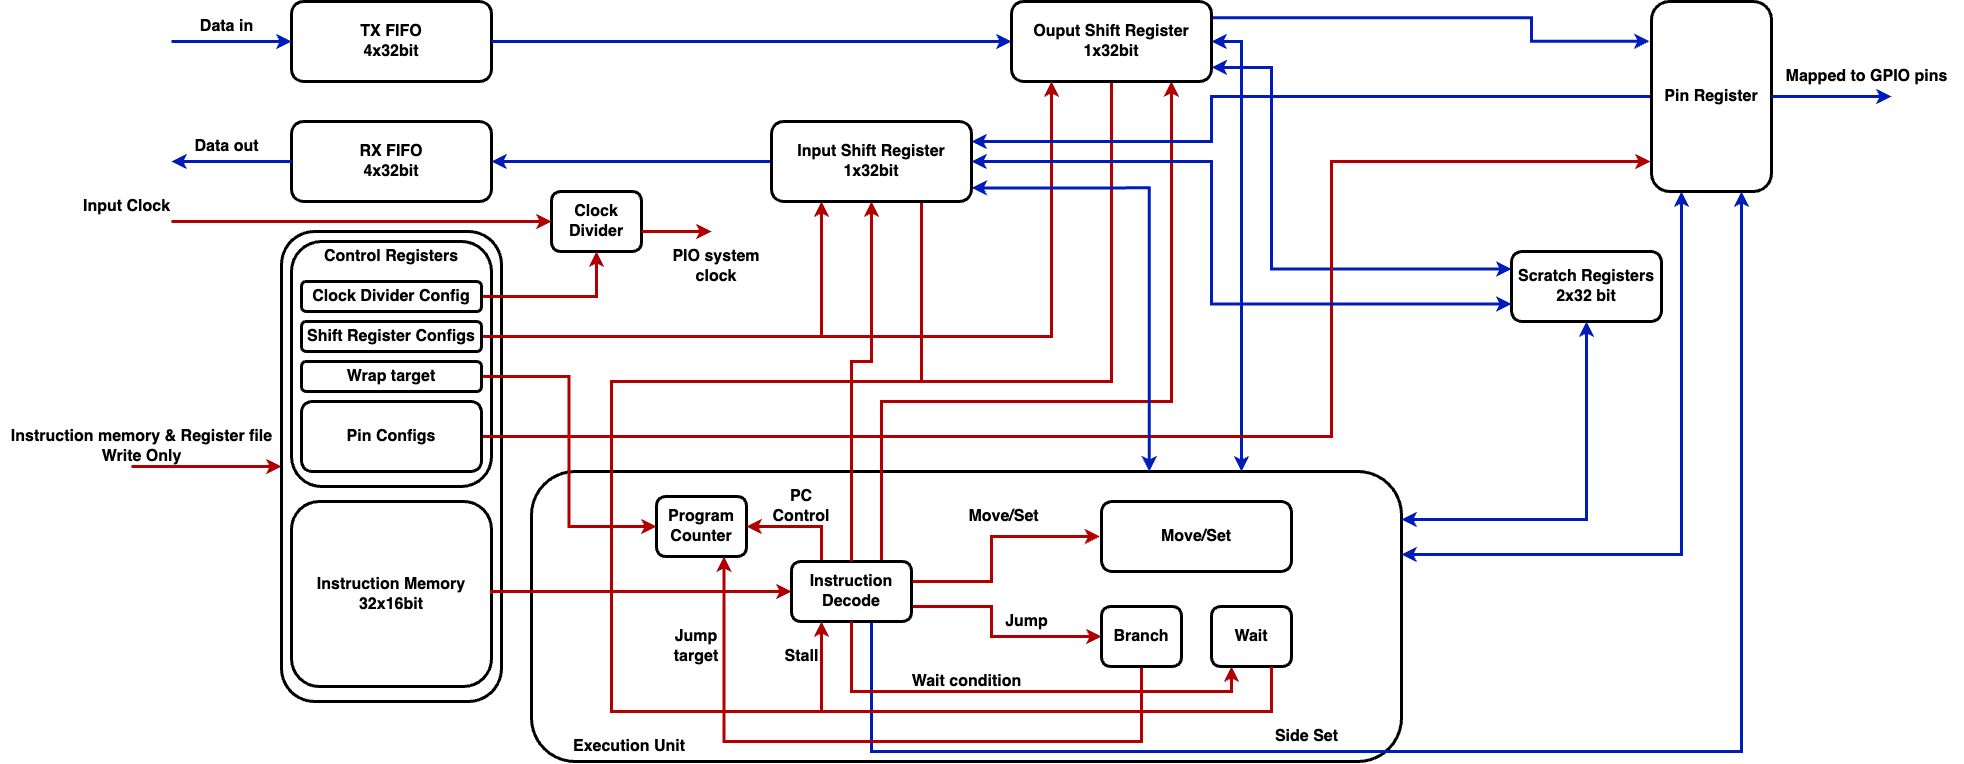
\includegraphics[width=0.9\textwidth]{../img/bd.png}
    \caption{The modular, hierarchical design of the PIO.}
    \label{fig:hdl_hierarchy}
\end{figure}

\section{PIO Components}
\subsection{Execution Unit}

The top-level execution unit wraps the decoder containing most of the logic with the three sub-execution units, which mostly contain very little logic and are wrapped as modules purely for hierarchical abstraction purposes. The module has read/write connections to all of the registers, which are all connected internally to the move module, which is just a big multiplexer between all the registers. The branch register also reads and writes from the registers, as the instruction set includes \txt{x++} and \txt{y++} as branch conditions, meaning that the execution unit includes logic to multiplex writes between those two units to the single write connection to the register.

The 5-bit program counter is also a sub-module of the execution unit. It's output is connected to the instruction memory's address input, and it is able to have a value written by the branch module. It automatically increments each cycle while it's \txt{incrementEnable} input line is high, which allows the instruction decoder to control it to implement delays and stalls.

\subsubsection{Instruction Decoder}

The implementation of the execution unit starts with the instruction decoder, which takes as input the instruction to be decoded, and asserts all the control signals required to execute that instruction. Most of the logic of the decoder is a series of \txt{when}/\txt{otherwise} statements, which are Chisel's equivalent of a behavioural \txt{if}/\txt{else} in Verilog. Listing \ref{lst:decoder} gives an example, where the first block is executed when the opcode is 0 to output the signals to the branch unit otherwise the outputs are all driven low. The mono-directional connection operator \txt{:=} is used to drive the outputs conditionally.

\begin{listing}[h!]
    \vspace{0.5cm}
    \begin{minted}{scala}
when(opcode === 0.U) {
    io.branchOp := instruction(7, 5)
    io.branchAddress := instruction(4, 0)
    io.branchEnable := true.B
}.otherwise {
    io.branchOp := 0.U
    io.branchAddress := 0.U
    io.branchEnable := false.B
}
    \end{minted}
    \caption{Sample code from the instruction decoder}
    \label{lst:decoder}
\end{listing}

The decode module is where delays and stalls are handled. If an instruction includes a delay, the module signals to the program counter not to increment to the next instruction, and the input instruction is substituted for a \txt{MOV null null} which acts as a no-op (\txt{NOP}). An input to the decoder also signals if the previous instruction caused a stall, either signalled externally from the execution unit via an input line or by a \txt{WAIT} instruction waiting on a condition, which will also cause the program counter not to increment and to re-execute the stalled instruction.

The side-set value is decoded within this module and asserted as an output. The side-set value is asserted before an instruction's delay cycles and regardless of whether it stalls or not, so the side-set value of an instruction must be latched such that the side-set of any \txt{NOP} instructions executed while sleeping (waiting for a delay to time out) do not take effect.

Ordinarily such logic would be representable by a D-type latch: the latch is transparent when enabled (not sleeping) and latches the side-set value when disabled, outputting the side-set value of the previous instruction. However, Chisel's timing model and implicit clocking does not make it easy to represent such logic. Synchronous register components are all based on flip-flops instead of latches, meaning that data is moved from input to output only on the rising clock edge

The code required to represent this in Chisel is shown in Listing \ref{lst:side-set}, and the equivalent circuit in Figure \ref{fig:side-set}. The \txt{RegEnable} object represents a single-bit register which is driven by the \txt{sideSet} signal (D goes to Q on the positive clock edge). The register is only write-enabled when the decoder is not in a delay cycle (represented by the \txt{sleeping} signal), and initialised to low on reset. The output side-set value \txt{io.sideSet} is driven by a multiplexer represented by a \txt{Mux} object, which outputs the value of the register if in a delay cycle, otherwise the value decoded directly from the instruction. This emulates a D latch, with the output being the input when not sleeping, and the stored value from the previous cycle when sleeping.

\begin{figure}[H]
    \centering
    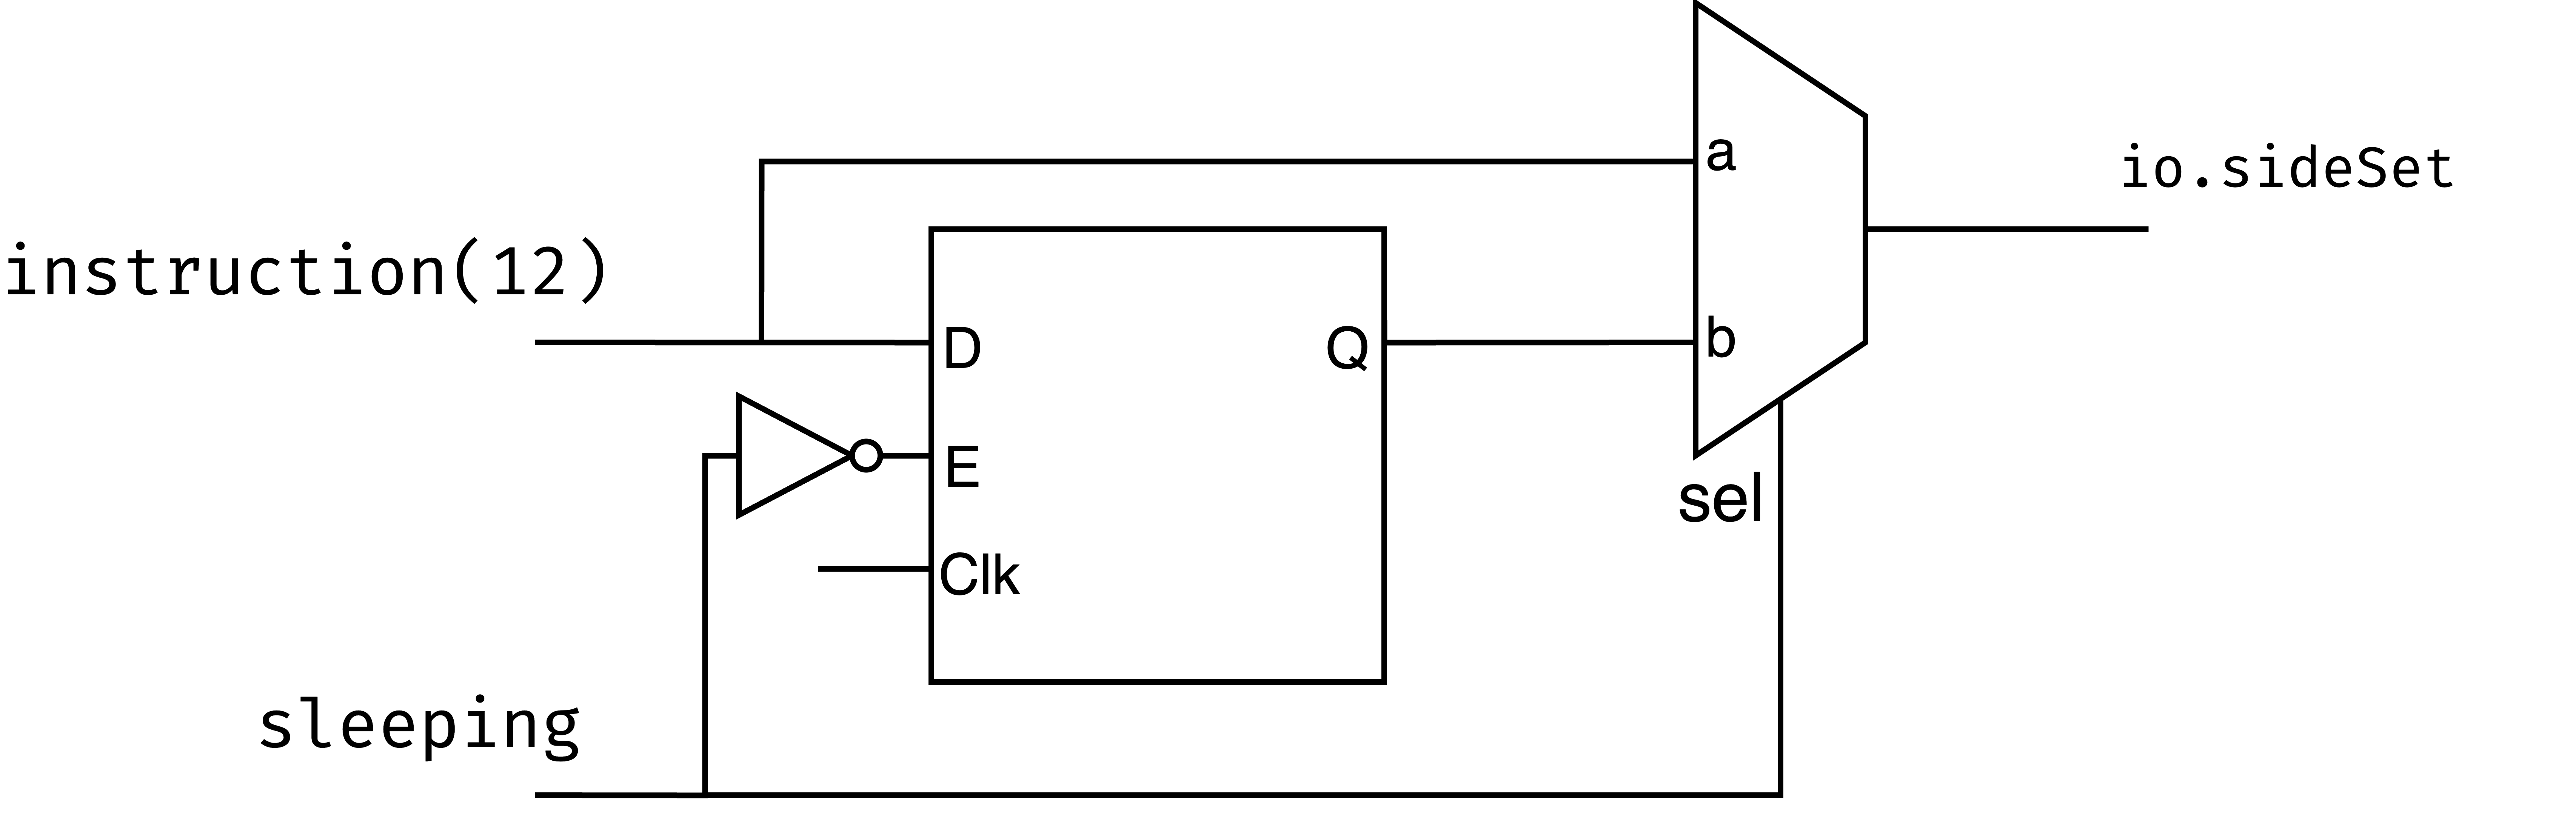
\includegraphics[width=0.9\textwidth]{../img/side-set.png}
    \caption{Logic for latching side-set}
    \label{fig:side-set}
\end{figure}

\begin{listing}[h!]
    \vspace{0.5cm}
    \begin{minted}{scala}
val sideSet    = instruction(12)
val sideSetReg = RegEnable(
    next = sideSet, 
    init = false.B, 
    enable = !sleeping
)
io.sideSet := Mux(sleeping, sideSetReg, sideSet)
    \end{minted}
    \caption{Chisel code for latching side-set}
    \label{lst:side-set}
\end{listing}

\subsection{FIFOs}

\subsection{Shift Registers}

\subsection{Pin Mapping}

\subsection{Other Components}

\section{AXI Wrapper}

\section{Chisel Abstractions}